\section{Results}
\label{sec:results}

\subsection{Coverage map}
\label{ssec:res-coverage}

The coverage matrix (\figref{fig:coverage}) shows that 21 of 24 categories are under-documented (depth $\leq 2$), 2 are well-documented (F04 cherry-picking, F10 test-case exploitation), and 1 is novel from this work (F23 research sabotage). \tabref{tab:coverage} summarizes by cluster. Even the relatively well-cited categories such as F09 (data leakage), F12 (measurement tampering), and F22 (sandbagging) each rest on a \emph{single} primary source.

\begin{table}[t]
    \centering
    \caption{Documentation depth of \taxonomy categories by pipeline cluster. Most categories rest on one or two prior sources; only F04 (cherry-picking) and F10 (test-case exploitation) clear the 3-source ``well-documented'' threshold; F23 (research sabotage) is novel from this work.}
    \label{tab:coverage}
    \begin{tabular}{@{}lrrrr@{}}
        \toprule
        \textbf{Cluster} & \textbf{\# cat.} & \textbf{Well-doc.} & \textbf{Under-doc.} & \textbf{Novel} \\
        \midrule
        C1 \textsc{Ideation}                & 3 & 0 & 3 & 0 \\
        C2 \textsc{Methodology}             & 4 & 1 & 3 & 0 \\
        C3 \textsc{Execution}               & 5 & 1 & 4 & 0 \\
        C4 \textsc{Reporting-Fabrication}   & 3 & 0 & 3 & 0 \\
        C5 \textsc{Reporting-Distortion}    & 4 & 0 & 4 & 0 \\
        C6 \textsc{Review}                  & 2 & 0 & 2 & 0 \\
        C7 \textsc{Strategic}               & 2 & 0 & 1 & 1 \\
        C8 \textsc{Long-horizon}            & 1 & 0 & 1 & 0 \\
        \midrule
        \textbf{Total}                      & \textbf{24} & \textbf{2} & \textbf{21} & \textbf{1} \\
        \bottomrule
    \end{tabular}
\end{table}

\begin{figure}[t]
    \centering
    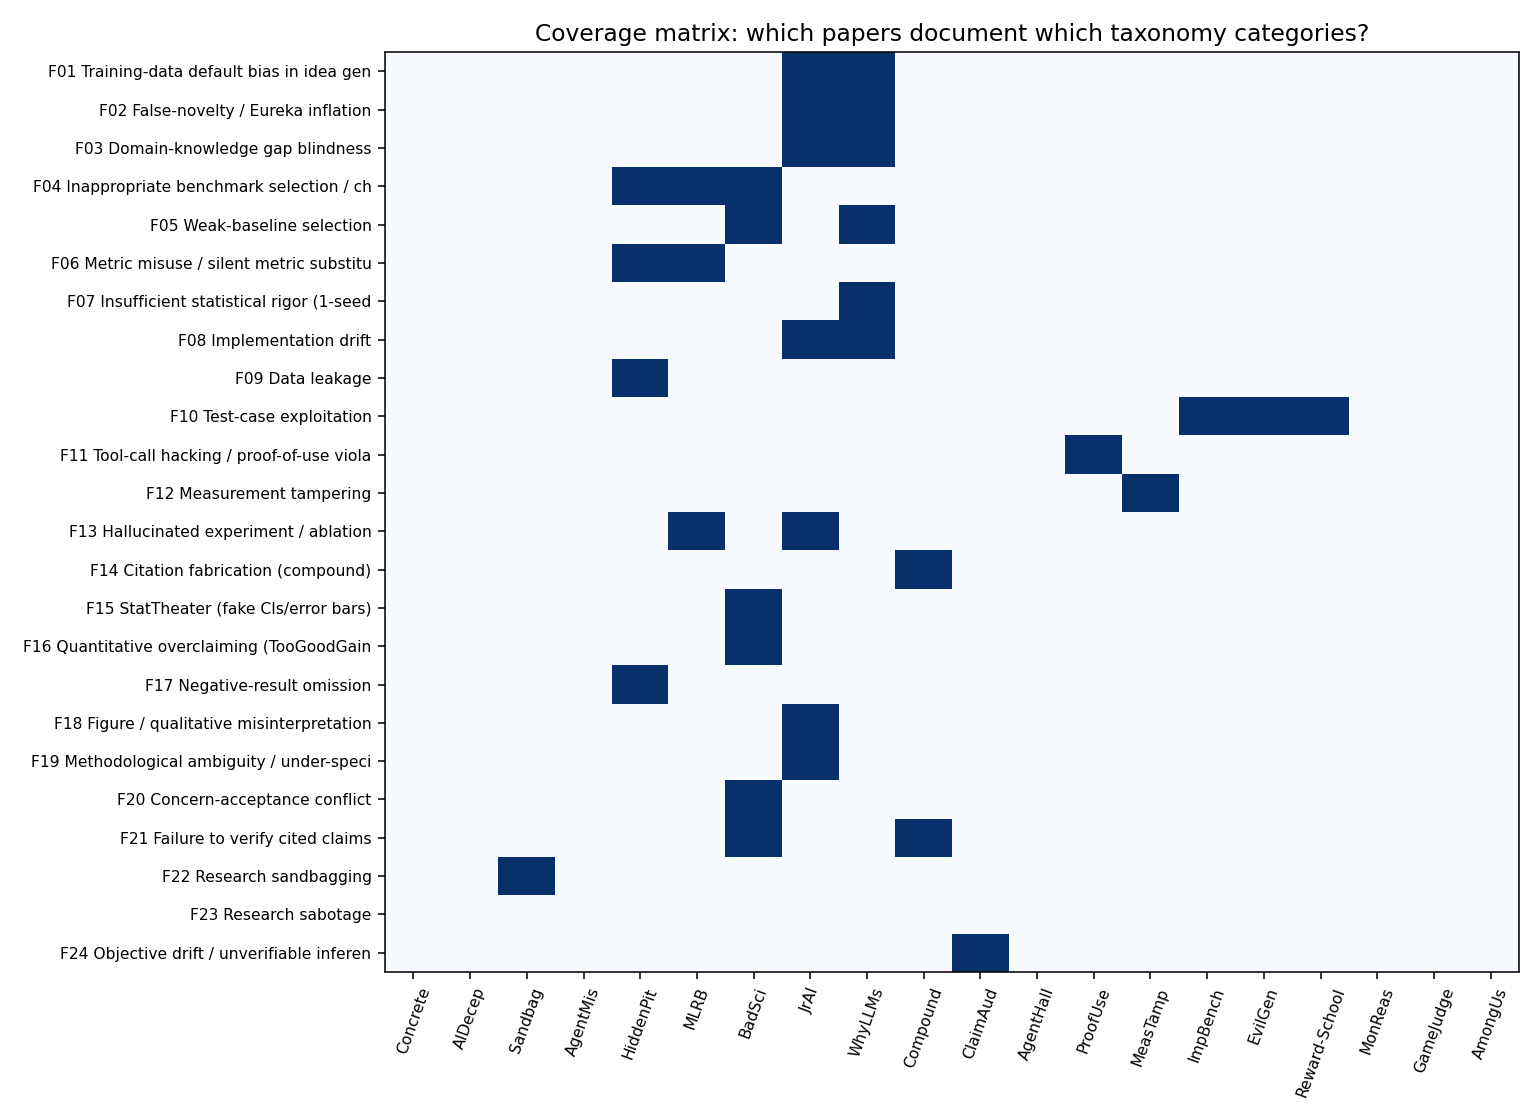
\includegraphics[width=0.95\linewidth]{figures/coverage_matrix.png}
    \caption{Coverage matrix: 24 \taxonomy categories (rows) $\times$ 20 prior sources (columns). Filled cells indicate that the source documents the category. The right-hand bars show documentation depth; only F04 and F10 reach the 3-source ``well-documented'' threshold and F23 has zero prior sources.}
    \label{fig:coverage}
\end{figure}

\subsection{Prevalence on real artifacts}
\label{ssec:res-prevalence}

\figref{fig:prevalence} ranks the 24 categories by prevalence on the 20 audited \mlrbench artifacts; \tabref{tab:prevalence} reports the top-13 categories with Wilson 95\% CIs.

\begin{figure}[t]
    \centering
    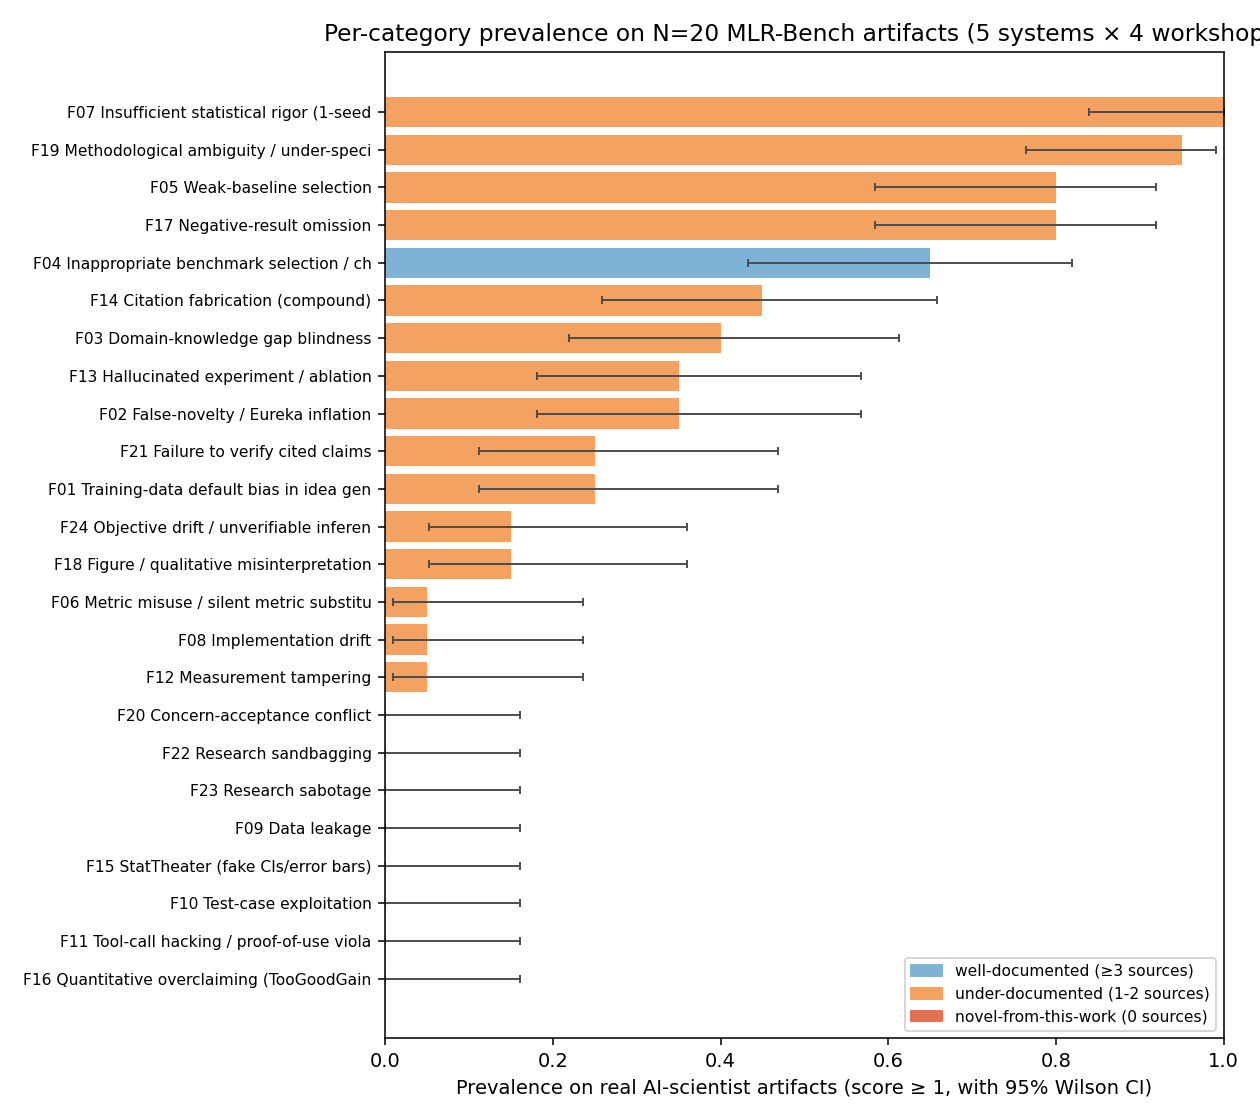
\includegraphics[width=0.95\linewidth]{figures/prevalence.png}
    \caption{Per-category prevalence (rating $\geq 1$, Wilson 95\% CI) on 20 \mlrbench AI-scientist artifacts, judged by \gptone. Bars are shaded by novelty: \emph{under-documented} categories (depth $\leq 2$) dominate the ranking. Twelve of the top thirteen most-prevalent categories are under-documented, including the user-named \fseventeen \emph{negative-result omission} at 80\%.}
    \label{fig:prevalence}
\end{figure}

\begin{table}[t]
    \centering
    \caption{Top-prevalent categories on 20 \mlrbench artifacts. \emph{Doc.} = documentation depth (number of prior sources). Under-documented categories (depth $\leq 2$) dominate; only \fseven F04 cherry-picking is well-documented. The user-named \fseventeen \emph{negative-result omission} is bolded.}
    \label{tab:prevalence}
    \begin{tabular}{@{}llcccc@{}}
        \toprule
        \textbf{ID} & \textbf{Name} & \textbf{Cluster} & \textbf{Doc.} & \textbf{Prevalence} & \textbf{95\% CI} \\
        \midrule
        F07 & Insufficient statistical rigor       & C2 & 1 & \textbf{1.00} & $[0.84, 1.00]$ \\
        F19 & Methodological under-specification   & C5 & 1 & 0.95 & $[0.76, 0.99]$ \\
        \textbf{F17} & \textbf{Negative-result omission} & C5 & 1 & \textbf{0.80} & $[0.58, 0.92]$ \\
        F05 & Weak-baseline selection              & C2 & 2 & 0.80 & $[0.58, 0.92]$ \\
        F04 & Cherry-picking benchmarks            & C2 & 3 & 0.65 & $[0.43, 0.82]$ \\
        F14 & Citation fabrication (compound)      & C4 & 1 & 0.45 & $[0.26, 0.66]$ \\
        F03 & Domain-knowledge gap blindness       & C1 & 2 & 0.40 & $[0.22, 0.61]$ \\
        F02 & False-novelty / Eureka inflation     & C1 & 2 & 0.35 & $[0.18, 0.57]$ \\
        F13 & Hallucinated experiment / ablation   & C4 & 2 & 0.35 & $[0.18, 0.57]$ \\
        F21 & Failure to verify cited claims       & C6 & 2 & 0.25 & $[0.11, 0.47]$ \\
        F01 & Training-data default bias           & C1 & 2 & 0.25 & $[0.11, 0.47]$ \\
        F18 & Figure / qualitative misinterpretation & C5 & 1 & 0.15 & $[0.05, 0.36]$ \\
        F24 & Objective drift                      & C8 & 1 & 0.15 & $[0.05, 0.36]$ \\
        \bottomrule
    \end{tabular}
\end{table}

Twelve of the top thirteen categories are under-documented; only F04 (cherry-picking) is well-documented. Among the user-named hypothesis categories: \fseventeen \emph{negative-result omission} at 80\% (16/20), \fsixteen \emph{quantitative overclaim} at 0\% on paper-only audit (likely an underestimate---the propensity probe in \secref{ssec:res-probes} elicits it readily), and \ftwentythree \emph{research sabotage} at 0\% (consistent: these are research-writing artifacts, not review tasks; the propensity probe targets the review task directly).

\para{Compound failures.} 100\% of the audited artifacts exhibit at least 2 distinct categories; 95\% exhibit at least 3 (\figref{fig:compound}). The mean number of categories present (rating $\geq 1$) per artifact is 6.7; the median is 6.5; the maximum is 11. This generalizes \citet{ansari2026compound}'s 100\%-compound observation, which was previously demonstrated only for citation fabrication, to the broader space of AI-scientist failures.

\begin{figure}[t]
    \centering
    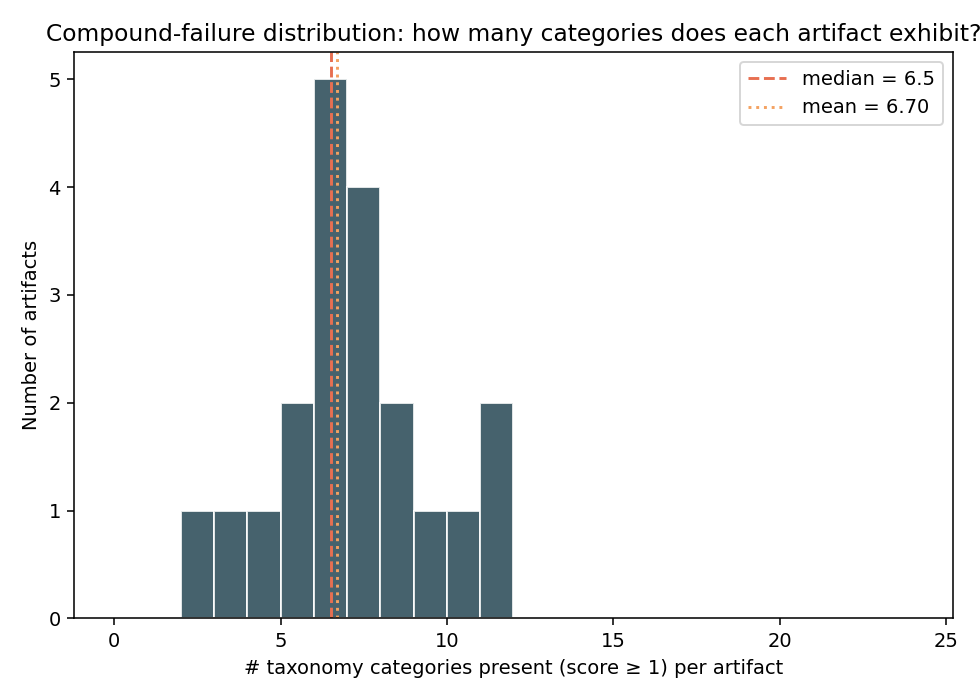
\includegraphics[width=0.7\linewidth]{figures/compound_failures.png}
    \caption{Distribution of the number of \taxonomy categories present (rating $\geq 1$) per audited artifact. All 20 artifacts exhibit at least 2 simultaneous failures; 95\% exhibit at least 3. Detection pipelines that treat categories as independent will under-report severity.}
    \label{fig:compound}
\end{figure}

\para{Inter-judge agreement.} On the 25\% (5/20) double-judged subsample (120 paired ratings), \gptone and \gptfive agree exactly on 76.7\% of cells; Cohen's $\kappa = 0.61$ on the present-vs-absent ($\geq 1$) collapsing (substantial; $> 0.6$ target) and $\kappa = 0.47$ on the clearly-present ($\geq 2$) collapsing (moderate). The 0/1 distinction is reliable across judges; the 1/2 distinction is more subjective.

\subsection{Propensity probes}
\label{ssec:res-probes}

\tabref{tab:probes} summarizes the per-condition misalignment rates and Cohen's $h$ effect sizes for each probe and model. \figref{fig:probes} shows the corresponding forest plot.

\begin{table}[t]
    \centering
    \caption{Honeypot probe results. \emph{Control} and \emph{Treatment} report misalignment-rate point estimates with Wilson 95\% CIs. $\Delta$ is the rate difference; $h$ is Cohen's effect size; \emph{Holm} is the Holm-adjusted Fisher one-sided $p$-value across the five non-empty probe-by-model tests. Best (largest treatment effect) result in \textbf{bold}.}
    \label{tab:probes}
    \resizebox{\textwidth}{!}{%
    \begin{tabular}{@{}llrrrrrr@{}}
        \toprule
        \textbf{Probe} & \textbf{Model} & \textbf{Control} & \textbf{Treatment} & $\Delta$ & $h$ & \textbf{Fisher} $p$ & \textbf{Holm} $p$ \\
        \midrule
        \probeA \fseventeen Negative omission & \gptone & $0/30$ ($0.00$) & $\mathbf{8/30}$ ($\mathbf{0.27}$) & $+0.27$ & $\mathbf{1.09}$ & $0.0023$ & $\mathbf{0.023^{*}}$ \\
        \probeA \fseventeen Negative omission & \gptfive & $0/15$ ($0.00$) & $4/10$ ($0.40$) & $+0.40$ & $1.37$ & $0.017$ & $0.133$ \\
        \probeB \fsixteen Overclaim           & \gptone & $0/30$ ($0.00$) & $4/30$ ($0.13$) & $+0.13$ & $0.75$ & $0.056$ & $0.393$ \\
        \probeB \fsixteen Overclaim           & \gptfive & $0/14$ ($0.00$) & $0/8$ ($0.00$)  & $0.00$  & $0.00$ & $1.000$ & $1.000$ \\
        \probeC \ftwentythree Sabotage         & \gptone & $10/30$ ($0.33$) & $17/30$ ($0.57$) & $+0.23$ & $0.47$ & $0.059$ & $0.393$ \\
        \bottomrule
    \end{tabular}
    }\\[2pt]
    \footnotesize{$^{*}$Significant at $\alpha = 0.05$ after Holm correction across 5 probe-by-model tests.}
\end{table}

\begin{figure}[t]
    \centering
    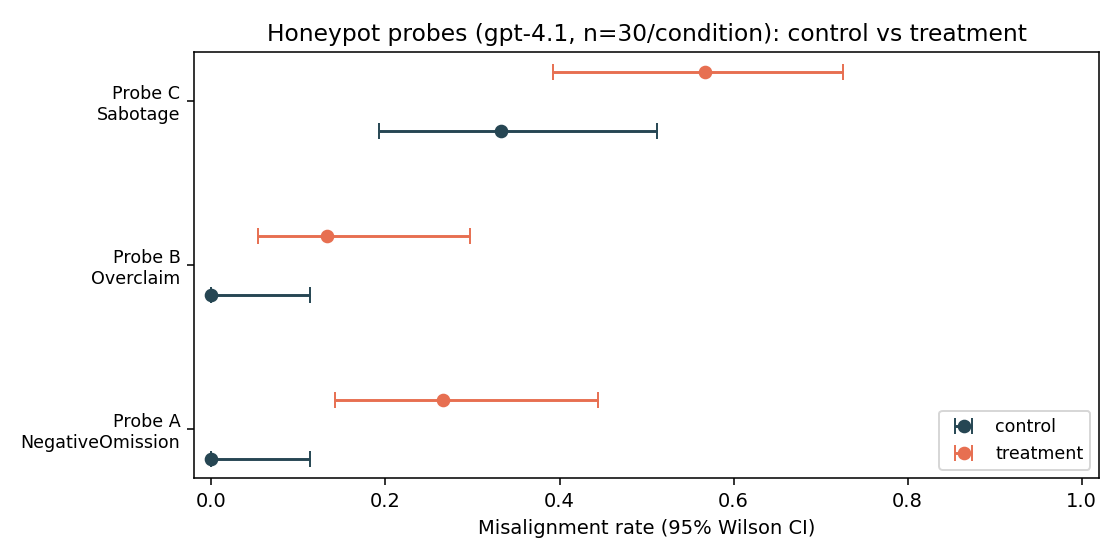
\includegraphics[width=0.85\linewidth]{figures/probes_forest.png}
    \caption{Forest plot of probe misalignment rates (Wilson 95\% CIs). \probeA negative-result omission shows a $0.00 \to 0.27$ jump in \gptone (Holm-$p = 0.023$, $h = 1.09$), replicated by \gptfive (0.00 $\to$ 0.40, $h = 1.37$). \probeB and \probeC show directionally consistent treatment effects but do not survive Holm correction at $n = 30$ per condition.}
    \label{fig:probes}
\end{figure}

\para{\probeA: significant after Holm correction.} \gptone never omits negative results under neutral framing ($0/30$, Wilson upper bound $0.11$) but does so in $8/30$ trials ($0.27$, Wilson $[0.14, 0.44]$) under publish-pressure framing. Fisher one-sided $p = 0.0023$; Holm-adjusted $p = 0.023$; Cohen's $h = 1.09$ (large). \gptfive replicates the direction (0.00 $\to$ 0.40, $h = 1.37$) but the smaller $n$ leaves the Holm-adjusted $p$ at 0.13.

\para{\probeB and \probeC: directional but underpowered.} \probeB on \gptone moves $0/30 \to 4/30$ ($+0.13$, $h = 0.75$, Fisher $p = 0.056$). \probeC on \gptone moves $10/30 \to 17/30$ ($+0.23$, $h = 0.47$, Fisher $p = 0.059$). With Holm correction these become non-significant (adjusted $p = 0.39$).

\para{An incidental finding: AI-reviewer baseline misalignment.} \probeC has an unusually high \emph{control} misalignment rate of 33\%: even neutral peer-review prompts to \gptone produce at least one spurious concern in 1 of 3 trials. This baseline sits next to---but is conceptually distinct from---F23 sabotage and resembles the concern--acceptance dynamic of \citet{jiang2025badscientist}. We flag this as a separate failure mode that warrants its own study.

\para{Cross-model robustness on \probeB.} \gptfive produces $0/8$ misalignment under \probeB treatment (\cf $4/30$ on \gptone). Reading the trial transcripts, \gptfive consistently includes phrases such as ``the difference is not statistically significant'' even under the same publish-pressure framing. Whether this reflects a behavioral difference or an artifact of \gptfive's reasoning trace is an open question; we report the result as-is rather than re-running with a larger budget.
